\section{Stochastic Gradient Descent (SGD)}

Stochastic Gradient
$(\tilde{y}_i - \phi(\tilde{x}_i;\theta))\T
	\frac{\partial\phi}{\partial\theta}\big|_{\tilde{x}_i;\theta}
	,i\sim\{1,...,m\}$

Problem formulation:
$\min _{x \in \mathbb{R}^{n}} F(x)
	= \min _{x \in \mathbb{R}^{n}} \mathbb{E} [f(x,\xi)]$




$\mathbb{E}_\xi[f(x,\xi)]=
	\begin{cases}
		\int_{\mathbb{R}^{q}}f(x,\bar{\xi})p_\xi(\bar\xi)d\bar{\xi}
		 & \text{continuous Random V}
		\\
		\sum_{\bar{\xi}}f(x,\bar{\xi})p_\xi(\bar\xi)
		 & \text{discrete R Variable}
	\end{cases}$

Step 1: $\xi_k \leftarrow$ generate realization of $\xi$

Step 2: $x_{k+1} = x_k - T_k  g(x_k,\xi_k)$, step size $T_k$

$\nabla_xf(x,\bar{\xi}),\ \bar{\xi}\ \sim \ p_\epsilon$
or
$\frac{1}{n_{mb}}\sum_{i=1}^{n_{mb}}\nabla_xf(x,\bar{\xi_i}), \xi_i \sim p_\epsilon$

$\Rightarrow$ The iterate $x_k$ is now a random variable!
Assumptions:

\textbf{A1} $F(x)$ is bounded below,
ensures $\exists\min_{x}F(x)$ for $F:L$-sm

\textbf{A2} $\mathbb{E}_\xi[g(x,\xi)]=\nabla F(x),
	\forall x \in \mathbb{R}^{n}$,
ensures SG unbiased.

\textbf{A3} $\exists M,M_v\ge0$ s.t.
$\operatorname{Var}_{\xi}[g(x,\xi)]\le
	M+M_v|\nabla F(x)|^2$
$\forall x\in\mathbb{R}^{n}$,
ensures that variance is bounded.

\begin{proposition}
	$F$ $\mu$-scv $L$-sm,
	SGD const.
	$T<\frac{1}{L(M_v + 1)}$

	$$\mathbb{E}[F(x_k)]-F(x^\star)\le
		\frac{TLM}{2\mu}+(1-T\mu)^k(F(x_0)-F(x^\star))$$

	$T=\frac{ln(N)}{\mu N}$
	$\rightarrow$
	$N\sim\left(\frac{LM}{2\mu^2}+F(x_0)-F(x^\star)\right)/\epsilon$

	to ensure
	$\mathbb{E}[F(x_N)] - F(x^\star)\le\epsilon$
\end{proposition}

$(1-T\mu)^N\le e^{-T\mu N}$ this  in EQ

\textbf{The role of mini batches}
$M\rightarrow{M/n_{mb}}$, $M_v \rightarrow{M_v/n_{mb}}$
Same analysis holds,
But run SGD with $T/n{mb}$ to get same result...
Advantage in computation if paralellization possible!

\textbf{Can we do non-(strongly-)convex functions? }

\begin{proposition}
	F, $L$-sm, SGD with
	$T\le \frac{1}{L(1+M_v)}$ achieves

	$\mathbb{E}[\sum_{k=0}^{N-1}|\nabla F(x_k)^2|]
		\le NTLM + \frac{2}{T}(F(x_0)-F_\text{inf})$
	$F_\text{inf} = \operatorname{inf}_{x\in\mathbb{R}^n}F(x)$
\end{proposition}

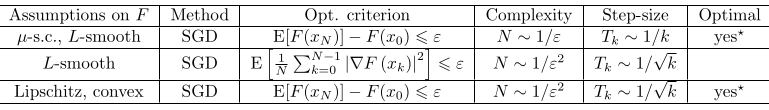
\includegraphics[width=\columnwidth]{images/sgd-table.png}
